\documentclass{beamer}
\usepackage{graphicx}
\usepackage{hyperref}

\title{FIONA Chatbot Application}
\author{Said Benaissa}
\date{\today}

\begin{document}

\frame{\titlepage}

\begin{frame}{Preventing Hallucinations and Providing Evidence}
    \begin{itemize}
        \item FIONA retrieves content directly from preloaded source documents stored in the backend.
        \item Embedding-based search using cosine similarity ensures accurate retrieval of relevant document chunks.
        \item Responses are generated using the `flan-t5-large` language model, including references to source documents.
        \item Prevents hallucinations by strictly relying on document embeddings and avoiding unsupported information.
    \end{itemize}
\end{frame}

\begin{frame}{CI/CD Pipeline for Document Changes}
    \begin{itemize}
        \item Monitors changes in both code and documents.
        \item Automatically rebuilds embeddings when documents are updated using `embedding_manager.py`.
        \item Redeploys the application to ensure up-to-date content and functionality.
        \item Ensures seamless integration of new information into the chatbot.
    \end{itemize}
\end{frame}

\begin{frame}{Deployment on Linux/Debian-based Systems}
    \begin{itemize}
        \item Docker Compose orchestrates backend and frontend services.
        \item Backend runs on `http://localhost:8000` and frontend on `http://localhost:3000`.
        \item Scalable deployment for small to large-scale systems.
        \item Fully on-premise deployment ensures data privacy.
    \end{itemize}
\end{frame}

\begin{frame}{Real-time User Interface}
    \begin{itemize}
        \item Clean and modern design built with React.
        \item Real-time responses to user queries in human language.
        \item Displays references to source documents for transparency.
        \item Visually appealing UI with responsive design for various devices.
    \end{itemize}
     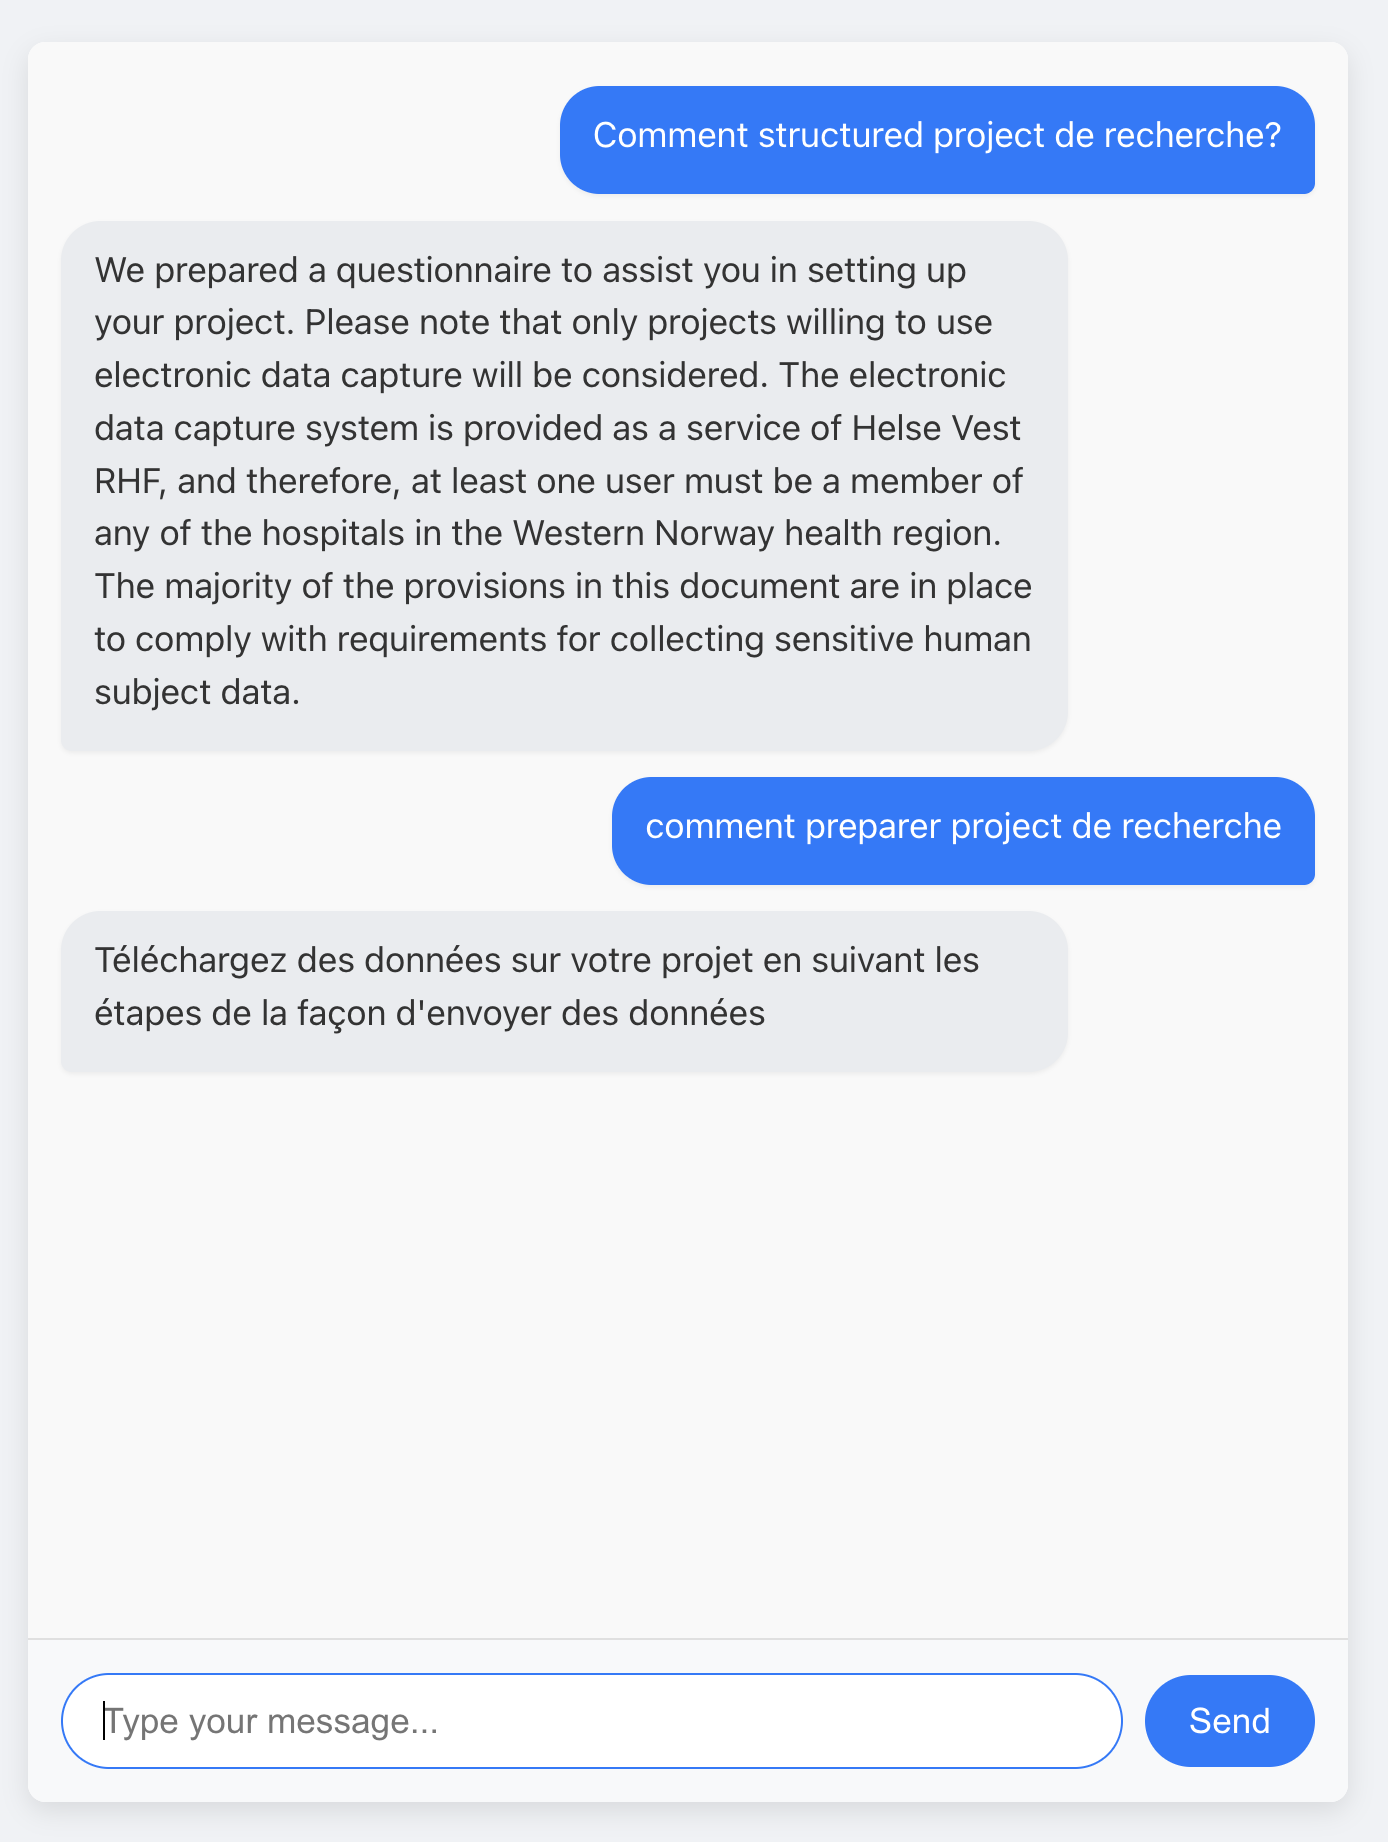
\includegraphics[width=\textwidth]{ui-screenshot.png} % Replace with an actual screenshot
\end{frame}

\begin{frame}{Integration with Apache2 and PHP 8.x}
    \begin{itemize}
        \item Backend can be proxied through Apache2 for seamless integration.
        \item Frontend served as static files compatible with PHP-based solutions (http://localhost:8080/index.php).
        \item Supports integration with existing enterprise systems using PHP 8.x.
        \item Ensures compatibility with legacy systems while maintaining modern features.
        \item Utilizes Apache2's mod_rewrite for clean URL handling.
    \end{itemize}
\end{frame}

\end{document}